\documentclass{sigchi}

% Use this command to override the default ACM copyright statement
% (e.g. for preprints).  Consult the conference website for the
% camera-ready copyright statement.

%% EXAMPLE BEGIN -- HOW TO OVERRIDE THE DEFAULT COPYRIGHT STRIP -- (July 22, 2013 - Paul Baumann)
% \toappear{Permission to make digital or hard copies of all or part of this work for personal or classroom use is      granted without fee provided that copies are not made or distributed for profit or commercial advantage and that copies bear this notice and the full citation on the first page. Copyrights for components of this work owned by others than ACM must be honored. Abstracting with credit is permitted. To copy otherwise, or republish, to post on servers or to redistribute to lists, requires prior specific permission and/or a fee. Request permissions from permissions@acm.org. \\
% {\emph{CHI'14}}, April 26--May 1, 2014, Toronto, Canada. \\
% Copyright \copyright~2014 ACM ISBN/14/04...\$15.00. \\
% DOI string from ACM form confirmation}
%% EXAMPLE END -- HOW TO OVERRIDE THE DEFAULT COPYRIGHT STRIP -- (July 22, 2013 - Paul Baumann)

% Arabic page numbers for submission.  Remove this line to eliminate
% page numbers for the camera ready copy
\pagenumbering{arabic}
% Load basic packages
\usepackage{balance}  % to better equalize the last page
\usepackage{graphicx} % for EPS, load graphicx instead
\usepackage{scrextend}
\usepackage{bera}% optional: just to have a nice mono-spaced font
\usepackage{listings}
\usepackage{xcolor}
\graphicspath{{figures/}}
\usepackage[T1]{fontenc}
\usepackage{txfonts}
\usepackage{mathptmx}
\usepackage[pdftex]{hyperref}
\usepackage{color}
\usepackage{booktabs}
\usepackage{textcomp}
% Some optional stuff you might like/need.
\usepackage{microtype} % Improved Tracking and Kerning
% \usepackage[all]{hypcap}  % Fixes bug in hyperref caption linking
\usepackage{ccicons}  % Cite your images correctly!
% \usepackage[utf8]{inputenc} % for a UTF8 editor only

% If you want to use todo notes, marginpars etc. during creation of your draft document, you
% have to enable the "chi_draft" option for the document class. To do this, change the very first
% line to: "\documentclass[chi_draft]{sigchi}". You can then place todo notes by using the "\todo{...}"
% command. Make sure to disable the draft option again before submitting your final document.
\usepackage{todonotes}

% Paper metadata (use plain text, for PDF inclusion and later
% re-using, if desired).  Use \emtpyauthor when submitting for review
% so you remain anonymous.
\def\plaintitle{Intelligent Tutor: Socratic Method Of Teaching}
\def\plainauthor{Christopher Bischke}
\def\emptyauthor{}
\def\plainkeywords{Intelligent Tutor; Socratic Method; Educational Technology}
\def\plaingeneralterms{Documentation, Standardization}

% llt: Define a global style for URLs, rather that the default one
\makeatletter
\def\url@leostyle{%
  \@ifundefined{selectfont}{
    \def\UrlFont{\sf}
  }{
    \def\UrlFont{\small\bf\ttfamily}
  }}
\makeatother
\urlstyle{leo}

% To make various LaTeX processors do the right thing with page size.
\def\pprw{8.5in}
\def\pprh{11in}
\special{papersize=\pprw,\pprh}
\setlength{\paperwidth}{\pprw}
\setlength{\paperheight}{\pprh}
\setlength{\pdfpagewidth}{\pprw}
\setlength{\pdfpageheight}{\pprh}

% Make sure hyperref comes last of your loaded packages, to give it a
% fighting chance of not being over-written, since its job is to
% redefine many LaTeX commands.
\definecolor{linkColor}{RGB}{6,125,233}
\hypersetup{%
  pdftitle={\plaintitle},
% Use \plainauthor for final version.
%  pdfauthor={\plainauthor},
  pdfauthor={\emptyauthor},
  pdfkeywords={\plainkeywords},
  bookmarksnumbered,
  pdfstartview={FitH},
  colorlinks,
  citecolor=black,
  filecolor=black,
  linkcolor=black,
  urlcolor=linkColor,
  breaklinks=true,
}

\colorlet{punct}{red!60!black}
\definecolor{background}{HTML}{EEEEEE}
\definecolor{delim}{RGB}{20,105,176}
\colorlet{numb}{magenta!60!black}

% create a shortcut to typeset table headings
% \newcommand\tabhead[1]{\small\textbf{#1}}

% End of preamble. Here it comes the document.
\begin{document}

\title{\plaintitle}

\numberofauthors{1}
\author{%
  \alignauthor{Christopher Bischke\\
    %\affaddr{for Submission}\\
    \affaddr{Boston, USA}\\
    \email{CBischke10@gmail.com}}\\
}

\maketitle

\begin{abstract}
  When looking at intelligent tutoring systems that help student’s study, there are many systems that act as a question-answer machine. The tutor will ask a question and the student will either provide the correct or incorrect answer. The tutor may give feedback depending on correctness, but other than the initial question, there is not much follow up for the student. What if the tutor challenged the student's assumptions? What if the student gives a correct answer to a question, but does not understand why it is the correct answer? This project is focused on building an intelligent tutoring system using the Socratic method of teaching. The Socratic method is used to keep questioning ideas and topics until the ultimate truth is understood and found.
\end{abstract}

%\category{H.5.m.}{Information Interfaces and Presentation
%  (e.g. HCI)}{Miscellaneous} \category{See
%  \url{http://acm.org/about/class/1998/} for the full list of ACM
%  classifiers. This section is required.}{}{}

\keywords{\plainkeywords}

  \section{Introduction}

  The Socratic method of teaching allows the teacher to question claims and ideas that the student assumed. The teacher is actually put into more of a subservient role to the student: where the teacher asks most, if not all the questions, and the student has to defend their claims. The Socratic method is named after the classical Greek philosopher, Socrates. Socrates is believed to be one of the founders of western philosophy. Socrates believed that all questions can be answered if students take a thoughtful disciplined approach to finding the ultimate truth \cite{Knox}. At a high level, the Socratic method allows students to get a deeper understanding on ideas through probing and continued questions.

  The learning objective for the Socratic method is inquiry. A teacher does not want to completely oppose the student’s original claims -- but ask a question that may alter their perspective on a claim or thought \cite{Dillon}. Next, which is critically important for the method, the learning session should be a dialog \cite{Dillon}. The teacher is supposed to ask questions and probe assumptions that the student may have made. And the student should answer questions and defend their claims based on their past experience and world knowledge. Finally the teacher asks questions that lead the student to the correct answer -- even though the student may keep answering questions incorrectly.
  
  An important component of the Socratic method of teaching is that the teacher is not a teacher in the traditional sense. The teacher is more of a guide on the student’s journey to truth -- rather than the teacher stating the truth. This allows the student to come to the conclusion of the answer on their own, which allows for a deeper understanding of the answer \cite{Bećirović}. According to  \cite{Bećirović}, the method can be broken down into five stages:
  \begin{enumerate}
  \item Wonder: an initial thought of why something the way it is. This could be a question to an assumption
  \item Hypothesis: An educated/formulated guess to the original wonder.
  \item Cross-examination: The students hypothesis is questioned. Is their hypothesis reasonable? Why did they guess this? Is there something that needs to be understood first?
  \item Acceptance or Rejection: After cross-examination, does the student accept or reject their hypothesis?
  \item Action: Acting on the findings \cite{Boghossian}. Does this lead to more wonder?
  \end{enumerate}
  \subsection{Benefits}
  The major benefit of this method is that it engages students. The natural setting for the Socratic method is a discussion. Immediately the student and teacher are considered more equals than the traditional teacher-student role. Remember the teacher’s role is just to ask questions and guide the student through the journey -- not state the ultimate truth. Since it is a discussion, the student and the teacher have a better understanding on how they respectively think about problems and solutions.
  
  Since the teacher is not a preacher and is involved in more of a dialog, there is a greater chance that the teachers learns as well. Since both the student and the teacher are in positions to learn, more ideas can be explored.
  
  \subsection{Drawbacks}
  The major drawback to the Socratic method is that it can be difficult to implement. At the least, the teacher needs to be disciplined in knowing when to ask questions and what questions to ask. At what point do you decide that a topic is exhausted and it is appropriate to continue onto another topic? This style of teaching can also be difficult for the teacher because they may have to ask a question that they themselves do not know the answer. As a teacher, that can be uncomfortable because teachers are usually looked upon as the ones that know all the answers.

  \subsection{Benefits of Automating the Socratic Method}
  Offering an automated tutor that can use different teaching styles can immensely benefit students and teachers in the classroom. As scaling classrooms and reaching more students can be its own challenge, so can finding teachers and assistants to aid students in learning. There exists learning tools that allow students to learn and test their knowledge based on a series of predefined questions and answers. Ultimately, these systems do not provide much dialog for the student.
  
  What if the student just memorized a general fact, but does not understand core underlying assumptions or evidence to a claim? A good Socratic teacher will continue to ask questions to a student even if they were correct in their original claim. An intelligent tutor that can enable students to critically think about problems can potentially offer higher quality of learning compared to simple correct-incorrect tutors. An intelligent tutor can scale with larger classrooms.

  \subsection{Problems Automating the Socratic Method}

  \begin{figure*}[!t]
  \centering
  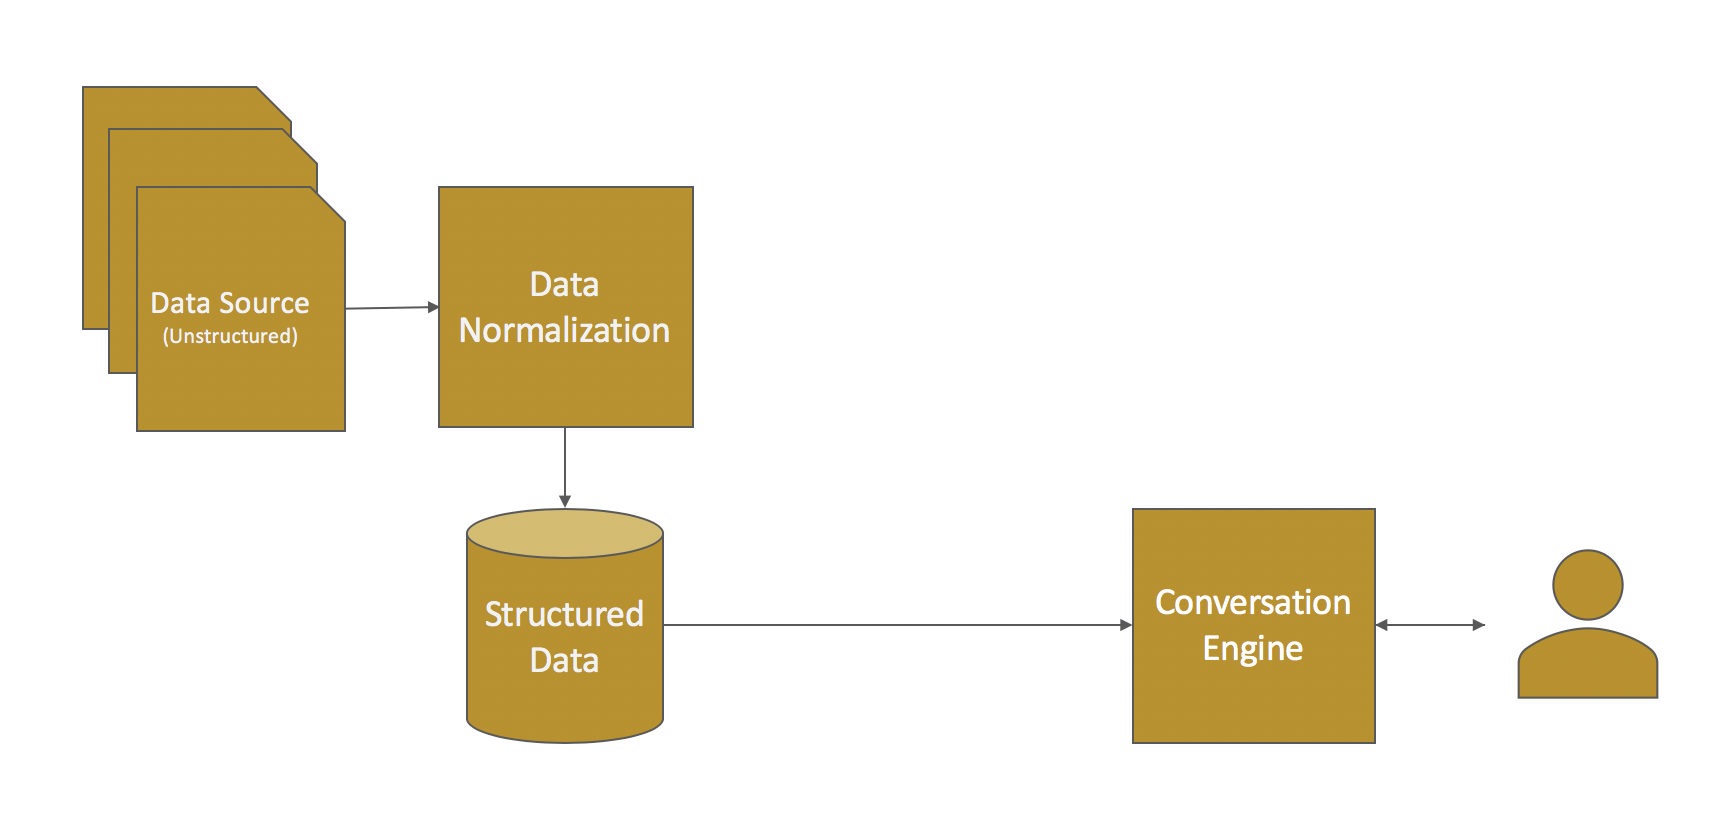
\includegraphics[width=6.0in]{high-level}
  \caption{High level data flow}
  \label{high-level}
  \end{figure*}

  From a high level algorithmic perspective, the Socratic method can decomposed into: identifying important learning objectives, conversing with students, and generating questions. Humans are easily able to identify and generate important questions while conversing with a student. However, one perspective could be that teachers have already digested a knowledge base and have pre generated questions before ever interacting with a student. If that is the case, then a machine just has to parse a knowledge base and identify the important topics. Once the important topics have been generated, then the machine has to interact with a student in a meaningful way that is Socratic. This project chooses a chat-bot interface to promote a conversation environment. The conversation with the student has to be as close to human like as possible to not distract from the Socratic method of learning.

  \section{Related Work}

  There are many different approaches for a tutor system for answering questions/studying for an exam. For instance, a website, justanswer.com will connect a student to a human that is a subject matter expert. The student may ask the tutor questions and the tutor explains ideas and concepts over chat. It is up to the tutor to decide how to answers questions. The tutor may simply answer the student’s question. Or the tutor may leverage any teaching methods to describe the answers. Since the tutor may use any approach, the student may be provided mentoring in the Socratic method. However; this solution is not automated and the Socratic method is not guaranteed.

  \cite{chen} offers a way to track knowledge mastery of topic to topic. By tracking the mastery, the tutor is able to offer new subjects to teach and learn. This also relates to this project because at some point the tutor needs to realize the answer is suffice and the ask a different question. However this approach does not give feedback in a Socratic method.

  AutoTutor is a dialogue system for interacting and teaching students \cite{AutoTutor}. AutoTutor seems to be the most similar to this project, but still does not provide tha guaranteed socratic experience. 

  
  \section{Methodology}

  \subsection{An Approach to Automating the Socratic Method}

  From a high level, the tutor is broken into four major components: Data source, data normalization, structured data, and the conversation engine. The data source acts as the knowledge base for the tutor. The data normalization pipeline translates unstructured text into structured data. The structured data is stored in such a way that the conversation engine only has to query to get relevant results and questions for the student.

  \subsection{Data Sources}
  
  The data source of this project is any unstructured text that explains a particular topic or idea. For example, a section of a Wikipedia article is an excellent input into the tutor. The idea is to find an unstructured text where all the knowledge is contained within the text but focused on a learning topic. Ideally, the sentences within the text should be grammatically correct. The tutor also cannot interpret any information or knowledge within a picture, figure, or chart. It is preferred that all pronouns are replaced with proper nouns to limit ambiguity for the tutor; However, in later chapters there are proposals on how to avoid this problem entirely.

  \subsection{Data Normalization and Structured Data}
  This component is responsible for converting the unstructured text into a meaningful structured knowledge. Most processing time is spent at data ingestion. This allows the conversation engine to quickly search for structured data and not have to spend precious processing time when interacting with the student. Consider a possible Socratic discussion between a student and mentor:

  \begin{addmargin}[1em]{2em}
    \textbf{Teacher:} How do we know that the earth is getting warmer? \\ 
    \textbf{Student:} Because I hear about it on the news. \\
    \textbf{Teacher:} How does the news know the earth is getting warmer? \\
    \textbf{Student:} Because the scientists say the earth is getting warmer. \\
    \textbf{Teacher:} How do the scientists know the earth is getting warmer? \\
    \textbf{Student:} Because they measure the temperature. \\
    \textbf{Teacher:} Do they just measure? Did they just start measuring temperature this year? \\
    \textbf{Student:} They must have measured the temperature of previous years then compared the temperatures year after year. \\
  \end{addmargin}

  In the above example, the first question, "How do we know that the earth is getting warmer?" can be considered the core question. For this project, a core question/idea is a general over arching idea that is made up of assumptions and axioms. From a lesson plan perspective, the core idea is the learning objective for the student. What happens when a student knows the answer to the core question? Does that mean the student has completed the learning objective? A student may not understand the underlying assumptions or reasons for the correct answer given. So continuing down the list of questions in the example are supporting ideas/questions that aid the student into realizing the ultimate truth for the core question -- with the final question being a very specific idea.
  
  The tutor in this project recreates this structure at the time of data ingestion: A core idea with supporting ideas. Each core idea and supporting ideas have questions and answers that allow the conversation engine to quickly fetch and ask a student a question. The idea is that the conversation engine should be performing minimal amount of natural language processing at the time of interacting with the student. This is because it is a time expensive process that could degrade the quality of interaction with the student.

  \subsection{Data Normalization Pipeline}

  \begin{figure*}[!t]
  \centering
  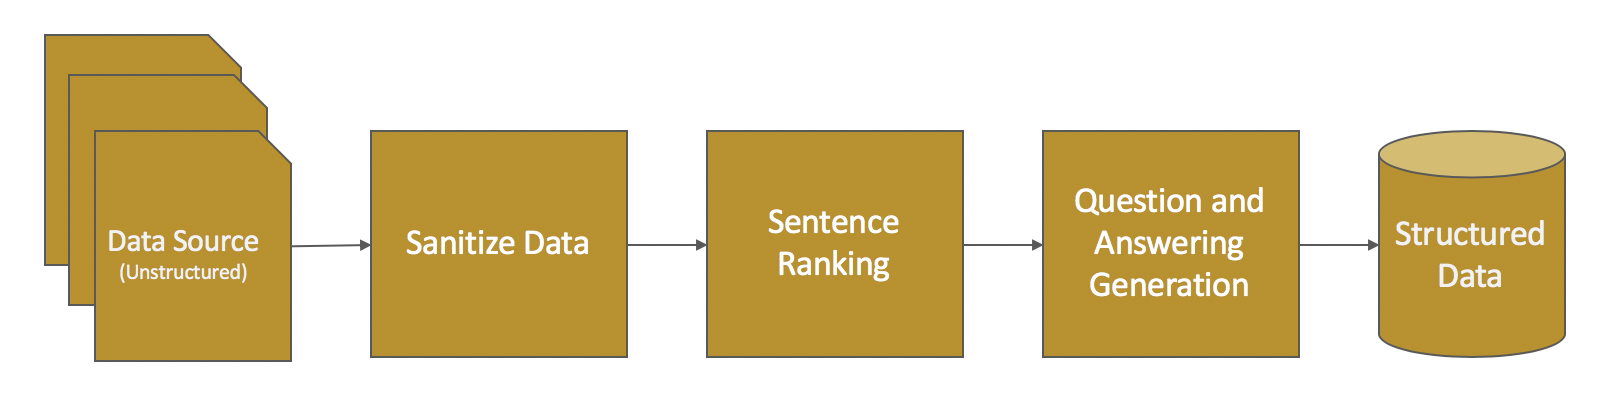
\includegraphics[width=6.0in]{normalization}
  \caption{Data ingestion data flow}
  \label{data-normalization}
  \end{figure*}

  The data normalization is a time expensive operation because this is where all the natural language processing and manipulation happens. At this point, the student is not interacting with the chat bot yet, so time is not a large concern for data normalization. The input to the normalization pipeline is assumed to be either a wikipedia article, text book, or scholarly source. The first step is to remove reference tags that could confuse the tagging of a sentence. Next, the tutor performs sentence tokenization, part of speech tagging, then sentence ranking.

  Sentence ranking is the main component for structuring the data in the format of core and supporting ideas. This project uses the LexRank algorithm for ranking sentences. LexRank is most commonly used for summarization of text automation \cite{LexRank}. LexRank is a graphed based approach for identifying relatively important sentences within a body of text. LexRank uses a connectivity matrix based on intra-sentence cosine similarity which is used as the adjacency matrix of the graph representation of sentences. This project sets the minimum similarity value a sentence pair must have to .85 (0-1). A higher similarity value means LexRank will grab not only relatively important sentences, but highly related sentences as well. After LexRank runs, the output is a ranking of sentences that are considered important and highly similar. The tutor stores the top ranked sentence as the core idea, and the following five sentences as supporting ideas. Below is an example of extracted core and supporting ideas from a Wikipedia article about Queen Elizabeth II:

  \begin{addmargin}[1em]{2em}
    \textbf{Core Idea:} She is the longest-lived and longest-reigning British monarch as well as the world's longest-reigning queen regnant and female head of state, the oldest and longest-reigning current monarch and the longest-serving current head of state. \\
    \textbf{Supporting Idea One:} In 2017, she became the first British monarch to reach a Sapphire Jubilee. \\
    \textbf{Supporting Idea Two:} Significant events have included her coronation in 1953 and the celebrations of her Silver, Golden, and Diamond Jubilees in 1977, 2002, and 2012 respectively. \\
    \textbf{Supporting Idea Three:} Elizabeth has occasionally faced republican sentiments and press criticism of the royal family, in particular after the breakdown of her children's marriages, her annus horribilis in 1992 and the death in 1997 of her former daughter-in-law Diana, Princess of Wales. \\
    \textbf{Supporting Idea Four:} However, support for the monarchy has consistently been and remains high, as does her personal popularity. \\
    \textbf{Supporting Idea Five:} Her many historic visits and meetings include a state visit to the Republic of Ireland and visits to or from five popes. \\
  \end{addmargin}

  Though the example above is not as clear as the global warming example presented earlier. It does seem that a teacher could easily generate questions with the ideas presented. The core idea does seem to be the most general and over arching, while the supporting ideas tend to be more specific.

  After ranking, the tutor now knows the important ideas of a text and supporting evidence. Now the tutor just needs to convert these ideas into questions. The tutor can generate and store questions before ever interacting with a student -- Again, this allows for fast fetching for the conversation engine.

  For each idea, the tutor generates questions based on Michael Heilman automatic factual question generation from text \cite{Heilman}. Heilman mostly uses a rule based approach to convert a sentences into a questions. For example, in the core idea presented above, a list of possible generated questions from Heilman's system are:

  \begin{addmargin}[1em]{2em}
    \textbf{Question One:} Who is the longest-lived and longest-reigning British monarch? \\
    \textbf{Question Two} Who is the longest-lived and longest-reigning British monarch as well as the world's longest-reigning queen regnant and female head of state, the oldest and longest-reigning current monarch and the longest-serving current head of state? \\
  \end{addmargin}

  However, Heilman's system does not provide answer generation for each question. This is why it is suggested to replace pronouns with proper nouns to reduce ambiguity of answer generation. For instance, if the tutor needs to generate the answer from the supplied sentence, the pronoun the referenced for the questions above would resolve to "she". In this case, no student would ever answer the question with she. There needs to be a coreference resolution to identify which pronouns refer to which proper nouns. There are many systems and algorithms that do that, but for the purpose of this project, the tutor will expect and assume an input where the proper noun is present.

  At this point, the tutor has stored core and supporting ideas and generated questions based on those ideas. The remaining components only have to interact with the structured text.


  \subsection{Conversation Engine}

  The conversation engine is in charge of fetching the appropriate structured data of the ingestion pipeline and providing an interface for the student. The interface for the student in this project is in the form of a chat bot. The chat bot knows the state of the conversation with the student. The chat bot asks a question within the supporting ideas, then depending on the correctness of the students answer, the tutor will ask a follow up question that is either more specific or general. The evaluation of the answer is based on a levenshtein distance of words of the student's answer to the answer stored in the structured data. This evaluation component can easily be replaced for any other comparison component. For the purpose of this project, the tutor judges any answer with a ratio of over .50 as correct.

  When the chat bot evaluates a question as correct or incorrect, the only feedback the student receives is another question. This is to promote the student to critically think about how the questions are linked and to find the answer themselves. When a student inquires about a topic, they will be asked questions until they have answered all the supporting questions. If the student begins to get questions incorrect, the student will be asked questions towards the core idea.
  \begin{figure*}[!t]
  \centering
  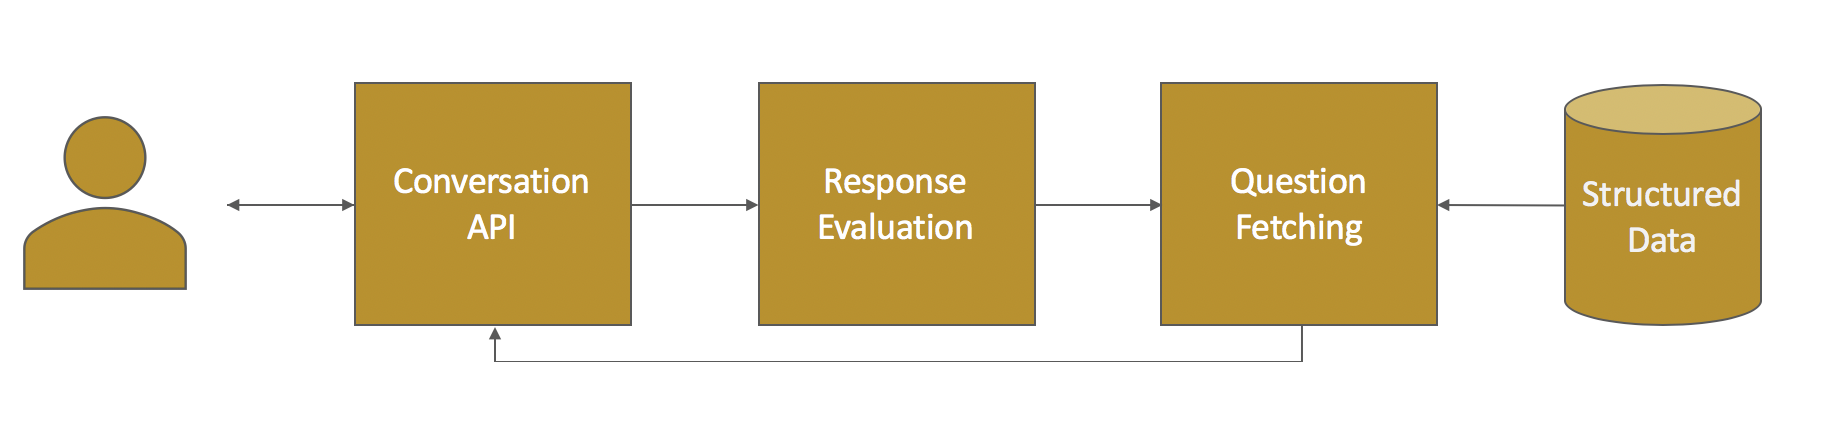
\includegraphics[width=6.0in]{conversation}
  \caption{The conversation engine dataflow}
  \label{conversation-flow}
  \end{figure*}

  \section{Architecture and Deployment}

  \begin{figure*}[!t]
  \centering
  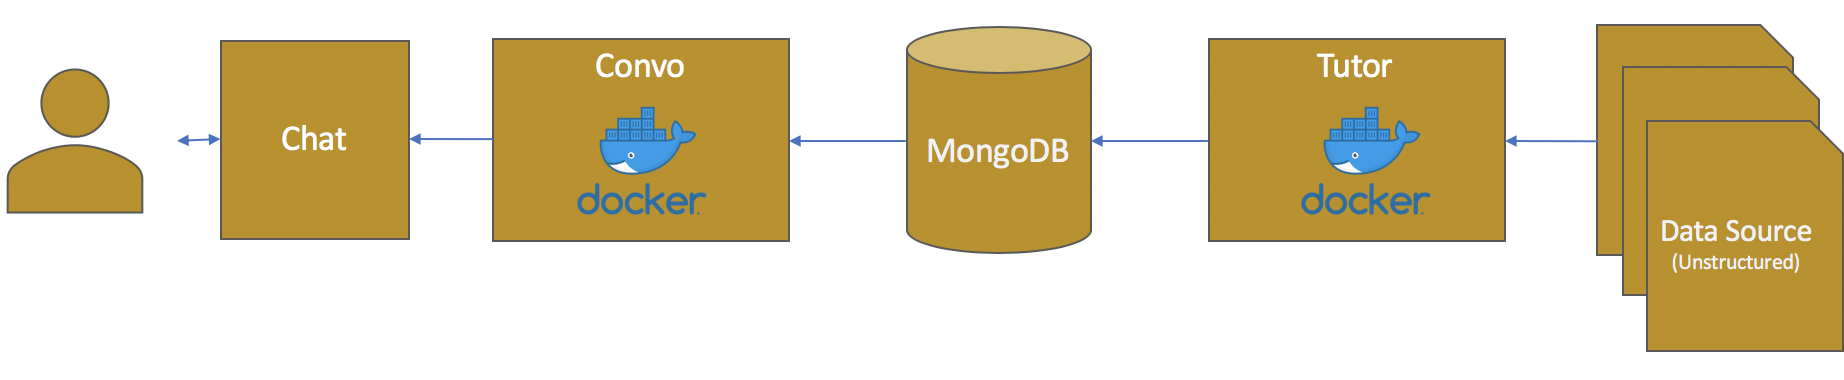
\includegraphics[width=6.0in]{deployment}
  \caption{Representation of the deployed docker containers and data flow}
  \label{deployment-flow}
  \end{figure*}

  This project is built mainly using Python. The question generation component is Java and all credit goes to\cite{Heilman}. Most of the natural language processing is done by Natural Language Toolkit (NLTK) \cite{nltk}. The code is built in five docker containers: Base, Tutor, Convo, Chat, and Mongo. The Base container holds similar dependencies for all other containers -- this allows for faster docker building and a reduction in physical space compared to installing similar dependencies on each container. The Tutor container houses the ingestion/normalization data pipeline. The Convo container houses the interface to interact with the structured data as well as the answer evaluation. Convo and Tutor are all RESTful interfaces. Finally the chat container houses the chat-bot for the student as well as logic that fetches questions from the convo container. The chat container is a server that can handle multiple users interacting with the same chat-bot; However, each user has their own session with the server. Finally the Mongo container houses the structured data for the Convo container to retrieve. The decoupling of the containers and responsibility is a choice to promote experimenting with different ideas more easily.

  \section{Future Work}

  The author's believe the most impactful improvements to this project would be implementing coreference resolution and sentence simplification. Coreference resolution would be used to help the question and answering generator to identify answers easily. The sentence simplification could help the question generator identify questions and answers easily. Following those two changes, the next steps would be to improve the evaluation service. Currently if there is an answer like "National Public Radio" and a student answers NPR, the tutor will evaluate that as incorrect.

  \section{Acknowledgments}


  The authors would like to thank David E. Wilson for his constant mentorship and encouragement. This project's success relied heavily on his patience, thoughtful feedback, and commuter rail counseling program.

  A special thanks to Michael Valete-Bischke for reminding the authors to have fun and not to take life or this project too seriously.
  
  \section{Conclusion}
  This project proves that the Socratic method in an intelligent tutor is possible. There is still work to be done in question generation and evaluation. This Socratic tutor could possibly help classrooms scale at a rate to reach more students without having to find more teachers or assistants. Code can be found at \url{https://github.gatech.edu/CBischke3/dunkin}

  \begin{thebibliography}{1}

  \bibitem{LexRank} 
  Erkan, G., Radev, D. R. (2004). LexRank: Graph-based Lexical Centrality as Salience in Text Summarization. Journal of Artificial Intelligence Research,22 457-479. doi:10.1613/jair.1523

  \bibitem{Dillon}
  Dillon, J. J. (2016). The Socratic Method. Teaching Psychology and the Socratic Method, 19-26. doi:10.1057/978-1-349-95050-8 3

  \bibitem{Heilman}
  Michael Heilman (2011). Automatic Factual Question Generation from Text. accessed \url{http://www.cs.cmu.edu/~ark/mheilman/questions/papers/heilman-question-generation-dissertation.pdf}

  \bibitem{AutoTutor}
  A. C. Graesser, P. Chipman, B. C. Haynes and A. Olney, "AutoTutor: an intelligent tutoring system with mixed-initiative dialogue," in IEEE Transactions on Education, vol. 48, no. 4, pp. 612-618, Nov. 2005. doi: 10.1109/TE.2005.856149 keywords: {intelligent tutoring systems;natural languages;distance learning;AutoTutor simulation;intelligent tutoring system;mixed-initiative dialogue;human tutor;natural language;animated conversational agent;3D interactive simulation;.NET framework;Intelligent tutoring systems;Natural languages;Conversational agents;intelligent tutoring systems;natural language dialogue;STEM learning;tutoring}

  \bibitem{Bećirović}
  Bećirović, Senad. (2016). Socratic Method as an Approach to Teaching. European Researcher. 111. 511-517. 10.13187/er.2016.111.511. 

  \bibitem{Knox}
  Knox D.K. (1998). Socrates: The First Professor. Innovative Higher Education, 23:2, 115-126.

  \bibitem{chen}
  Chen Tainjin. (2017) Improve Cognitive Tutoring By Designing Knowledge Mastery Tracking Based Course using OPPIA. Retrieved October 2018 from \url{https://github.gatech.edu/kbrunson6/6460_papers/blob/master/papers/iZNEG9Oh.pdf}

  \bibitem{nltk}
  Bird, Steven, Edward Loper and Ewan Klein (2009), Natural Language Processing with Python. O’Reilly Media Inc.

  \bibitem{Boghossian}
  Boghossian, P. (2012). Socratic Pedagogy: Perplexity, humiliation, shame and a broken egg. Educational Philosophy and Theory, 44:7, 710-720.


  
    \end{thebibliography}


  % that's all folks
  \end{document}